% f2015gdw_q15_circle.tex — 2015 年高考数学·广东卷·文科 第 15 题（圆与切线）
%
% 【来源】`.work/phase3-b16/source/2015广东文.pdf`（SHA-256
%   0c27f1a08f837014066c636a3190b8fa7ad7e5a4494f204e60412293aea17e09），
%   第 1 页（合订本页 949）第 2 栏；内容对象 5。逐路径实测见
%   `.work/phase3-b16/figure-inventory.md` Q15 节。
%
% 【坐标口径】清单坐标为「真页 pt、原点左上、y 向下」。本图取
%   X0 = 526.4664（圆最左点 x），Y0 = 398.4110（圆最低点 y_top），
%   本地坐标  (x, y) = (x_page − X0, Y0 − y_top)，
%   即本地 x 向右、y 向上，1 单位 = 1 TeX pt；tikzpicture 用 x=1pt, y=1pt。
%   换算示例：圆心 (571.5954, 353.2830) → 本地 (45.1290, 45.1280)；
%   A (526.4672, 353.2830) → (0.0008, 45.1280)；E (661.8502, 353.2830) → (135.3838, 45.1280)。
%   清单中的真页坐标逐点写在每题注释里，便于反查。
%
% 【线宽/虚线】全部路径 line width = 0.398pt（源内容流 `0.398 w`）；无虚线。
%   圆为 4 段三次贝塞尔（不是 arc 算子）：控制点距端点 24.92pt，
%   κ = 24.92 / 45.125 = 0.55225，与标准 κ 一致（FI-S7）。
%
% 【照源复刻的存疑项】
%   FI-S6：切点 C = (594.16, 314.20) 不是折线顶点；DE 为整段直线，
%          标签 C 基线 (594.96, 312.86) 相对切点偏移 (+0.80, −1.34) pt，照录。
%   FI-S7：圆用 4 段三次贝塞尔路径级复现，不用 \draw circle 近似。
%   圆心点：源为 CMSY10 0x0F（`\bullet`）文本字形，文本矩阵含 0.6 缩放
%          （CMSY10 10.5pt × 0.6 = 6.3pt 有效），基线原点 (570.0200, 354.6828)；
%          此处用 node scale=0.6 复现同一缩放（实测 1200dpi 墨径 2.40pt，
%          与源 2.46pt 一致），非矢量圆点。不用 \fontsize{6.3pt}——那会
%          触发 CMSY6 光学字号替换，墨径偏大（2.82pt）。
%
% 【自验结果】见文件末尾。
%
% 元素计数：4 条路径（1 圆 = 4 段贝塞尔 + 3 直线段）、7 个标签
%   （A B C D E O + 圆心点）。
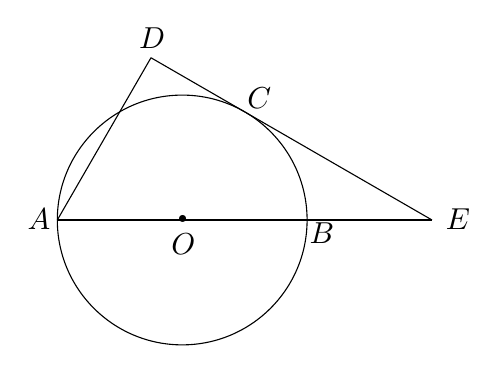
\begin{tikzpicture}[x=1pt, y=1pt,
    every node/.style={inner sep=0pt, font=\fontsize{10.5pt}{12.6pt}\selectfont}]

  % ---- 圆：m + 4c + h（源内容流 path 20，lw 0.398） ----
  % 源真页坐标：m (616.7234,353.2830)
  %   c (616.7234,328.3590) (596.5194,308.1550) (571.5954,308.1550)
  %   c (546.6714,308.1550) (526.4664,328.3590) (526.4664,353.2830)
  %   c (526.4664,378.2070) (546.6714,398.4110) (571.5954,398.4110)
  %   c (596.5194,398.4110) (616.7234,378.2070) (616.7234,353.2830)  h
  \draw[line width=0.398pt]
    (90.2570,45.1280)
    .. controls (90.2570,70.0520) and (70.0530,90.2560) .. (45.1290,90.2560)
    .. controls (20.2050,90.2560) and (0.0000,70.0520) .. (0.0000,45.1280)
    .. controls (0.0000,20.2040) and (20.2050,0.0000) .. (45.1290,0.0000)
    .. controls (70.0530,0.0000) and (90.2570,20.2040) .. (90.2570,45.1280)
    -- cycle;

  % ---- 垂线 AD（源 path 21，lw 0.398）：A(526.4672,353.2830) → D(560.3132,294.6600) ----
  \draw[line width=0.398pt] (0.0008,45.1280) -- (33.8468,103.7510);

  % ---- 直径延长线 AE（源 path 22，lw 0.398）：A(526.4672,353.2830) → E(661.8502,353.2830) ----
  \draw[line width=0.398pt] (0.0008,45.1280) -- (135.3838,45.1280);

  % ---- 切线 DE（源 path 23，lw 0.398）：D(560.3131,294.6605) → E(661.8501,353.2835) ----
  \draw[line width=0.398pt] (33.8467,103.7505) -- (135.3837,45.1275);

  % ---- 标签：源文本 Tm 原点（基线左端），CMMI10 10.5pt ----
  \node[anchor=base west] at (-10.9104,41.5400) {$A$};   % 源 (515.5560,356.8710)
  \node[anchor=base west] at (90.9416,36.6090)  {$B$};   % 源 (617.4080,361.8020)
  \node[anchor=base west] at (68.4956,85.5540)  {$C$};   % 源 (594.9620,312.8570)
  \node[anchor=base west] at (29.3546,107.1370) {$D$};   % 源 (555.8210,291.2740)
  \node[anchor=base west] at (140.1726,41.5400) {$E$};   % 源 (666.6390,356.8710)
  \node[anchor=base west] at (40.9786,32.5740)  {$O$};   % 源 (567.4450,365.8370)
  % 圆心点：源 CMSY10 0x0F（`\bullet`），Tm 为 0.6 缩放（CMSY10 10.5pt × 0.6），
  % 基线原点 (570.0200,354.6828) → 本地 (43.5536,43.7282)。
  \node[anchor=base west, scale=0.6] at (43.5536,43.7282) {$\bullet$};

\end{tikzpicture}
%
% 【自验结果】
%   探针：latexmk -pdfxe，0 error / 0 Overfull / 0 Underfull / 0 Missing character；
%         页面 162.34 × 114.08 pt（standalone border=0）。
%   tex 反算：4 条路径 + 7 个标签全部匹配，最大残差 0.000000 pt（阈值 0.05）。
%   600dpi 墨迹：整体墨迹包围盒最大边差 0.188 pt；几何包围盒 0.124 pt；
%         标签中心最大 0.240 pt（D）。（以上为尺度归一值，已扣除探针
%         0.996277 = 72/72.27 的 TeX pt / PDF bp 均匀因子）
%         按页面 bp 直接比较（物理）最大 0.604 pt，全部来自该 0.37% 均匀缩放。
%   灵敏度：端点 E +0.15pt → tex 检查器报 0.1500、600dpi 几何包围盒报 0.2409；
%         标签 C +0.15pt → tex 检查器报 0.1500、600dpi 标签中心报 0.1204。均能报出。
